\documentclass[11pt]{article}

% Build with XeLaTeX + Biber (see build.ps1).
\usepackage{fontspec}
\usepackage[a4paper,margin=25mm]{geometry}
\usepackage{graphicx}
\usepackage{booktabs}
\usepackage{amsmath}
\usepackage{siunitx}
\usepackage{xcolor}
\usepackage{caption}
\usepackage[colorlinks=true,linkcolor=black,citecolor=blue,urlcolor=blue]{hyperref}
\usepackage[backend=biber,style=numeric,sorting=none]{biblatex}
\addbibresource{references.bib}

\captionsetup{font=small,labelfont=bf}
\graphicspath{{figures/}}

\title{\textbf{Yertle: Learned Locomotion for a Low-Cost 3D-Printed Quadruped}\\
\large From a Hand-Tuned Gait to Reinforcement Learning and Sim-to-Real}
\author{Jerome Graves}
\date{2026}

\begin{document}
\maketitle

\begin{abstract}
\noindent
Yertle is an open-source, 3D-printed, twelve degree-of-freedom quadruped built
from hobby servos at a hardware cost of around \pounds 250. This report describes
its progression from a hand-tuned sinusoidal gait to learned locomotion trained
with deep reinforcement learning, together with a path to deployment on the
physical robot. Two independent training pipelines are presented: a CPU pipeline
using PyBullet and Proximal Policy Optimization, and a GPU pipeline using NVIDIA
Isaac Lab with thousands of parallel environments. The Isaac Lab pipeline learns
a velocity-tracking walking policy in about ten minutes on a single consumer GPU,
reaching full-length episodes (the robot does not fall) while tracking commanded
body velocities. A sim-to-real deployment bridge and a ROS 2 node are described
that turn a trained policy into joint commands for the on-board microcontroller.
The report also documents the practical engineering that such a project requires,
including physics-model repair, reward shaping, and a set of Windows-specific
issues encountered when running the simulators.
\end{abstract}

\section{Introduction}
Legged locomotion has moved decisively toward learning-based control. Policies
trained in simulation and transferred to hardware now walk, run, and recover on
real quadrupeds \cite{hwangbo2019anymal}, and the availability of massively
parallel GPU simulation has reduced training time from days to
minutes \cite{rudin2022minutes}. Most demonstrations, however, use expensive
research platforms. This work applies the same modern stack to \emph{Yertle}, a
cheap, printable quadruped, and takes it end to end: from a mechanism and
firmware through two reinforcement-learning pipelines to a deployable controller
and a ROS 2 interface.

The contributions are practical rather than novel in method. They are: (i) a
clean, reproducible reinforcement-learning environment for a low-cost quadruped,
provided in both a CPU (PyBullet) and a GPU (Isaac Lab) form; (ii) a trained
velocity-tracking walking policy and the artifacts to reproduce it; (iii) a
sim-to-real bridge and a ROS 2 node that connect the learned policy to the
existing firmware; and (iv) an honest account of the engineering obstacles, which
are usually omitted from polished results but dominate the real effort.

\section{System Overview}
Yertle consists of four legs, each with three degrees of freedom driven by hobby
servos, giving a leg extension of roughly \SI{20}{\centi\meter} and a total mass
near \SI{1.8}{\kilogram}. An ESP32 microcontroller running FreeRTOS handles the
servo bus (through a PCA9685 driver), reads a nine-axis inertial measurement
unit, and communicates over WiFi or serial. One core computes inverse kinematics
and drives the servos; the other handles communication. A host computer sends
either joint angles or Cartesian foot targets, and the firmware executes them.
The original control software is a Python GUI that generates a sinusoidal trot by
hand. The work described here replaces that hand-tuned gait with a learned policy.

\section{Simulation Model}
Both pipelines share the same kinematic description, a URDF exported from the CAD
model. Preparing this model for physics simulation required two fixes that are
representative of the practical work involved.

\paragraph{Inertia.} The exported URDF specified physically invalid inertia
tensors: zero inertia on the base link and, on the leg links, off-diagonal terms
equal to the diagonal terms. A valid rigid-body inertia tensor must be symmetric
positive-definite. PyBullet tolerates the invalid values by silently
recomputing, but the PhysX engine used by Isaac Lab rejects them for articulated
bodies. Each tensor was replaced with a stable, mass-scaled diagonal estimate.

\paragraph{Mesh naming.} Four mesh files contained spaces in their names. This is
harmless for PyBullet but illegal in the prim-path syntax used by Universal Scene
Description (USD), so the conversion to USD failed until the files were renamed.

For the GPU pipeline the corrected URDF is converted to USD with Isaac Lab's
importer, merging the fixed base joint and producing an articulation with a
\texttt{base\_link} root and twelve revolute joints.

\section{Method}
\subsection{Reinforcement-learning formulation}
Locomotion is posed as velocity-command tracking. At each control step the policy
observes the base linear and angular velocity, a projected-gravity vector (which
is an inertial-measurement-style estimate of the down direction), the commanded
body velocity, the joint positions and velocities, and the previous action. The
action is a set of twelve target joint angles, applied as offsets around a fixed
standing pose and tracked by a position controller. This choice mirrors the real
robot, which is commanded with joint angles, and keeps the sim-to-real gap small.
The reward rewards tracking of the commanded planar and yaw velocities while
penalizing falling, energy use, action rate, and body tilt.

\subsection{CPU pipeline: PyBullet and PPO}
The first pipeline wraps the URDF in a Gymnasium \cite{towers2023gymnasium}
environment with a PyBullet \cite{coumans2021pybullet} backend and trains with
Proximal Policy Optimization \cite{schulman2017ppo} using
Stable-Baselines3 \cite{raffin2021sb3}. Domain randomization over base mass, foot
friction, sensor noise, and random pushes \cite{tobin2017domainrand} is applied
per episode to encourage transferable behavior. This pipeline runs on any
machine without a GPU and is intended as a portable, reproducible reference.

A useful lesson emerged here. An early reward function drove the policy to a
degenerate optimum in which it stood perfectly still: the survival and stability
terms, combined with a forgiving velocity-tracking kernel and command ranges that
included near-zero speeds, made standing near-optimal. The fix was to add a direct
forward-progress term, sharpen the tracking kernel, require a non-trivial
commanded speed, and add an entropy bonus for exploration. This is a
representative example of reward shaping and of the value of \emph{evaluating}
a policy rather than trusting the reward curve alone.

\subsection{GPU pipeline: Isaac Lab and rsl\_rl}
The second pipeline uses NVIDIA Isaac Lab \cite{mittal2023orbit}, built on Isaac
Sim and the PhysX engine, which simulates thousands of environments in parallel on
a single GPU \cite{makoviychuk2021isaacgym}. The Yertle articulation is dropped
into Isaac Lab's velocity-tracking locomotion task, the same task used to train
research quadrupeds, with body names remapped to Yertle's and terrain and command
ranges scaled for a small robot. Training uses the \texttt{rsl\_rl} implementation
of PPO \cite{rudin2022minutes}. A flat-ground task and a rough-terrain task (which
adds procedurally generated terrain and a height scanner) are both provided.

\section{Results}
The GPU pipeline was trained on a single NVIDIA GeForce RTX 4070 with 4096
parallel environments. Training throughput was approximately 80{,}000 simulation
steps per second, roughly two orders of magnitude faster than the single-process
CPU pipeline. A walking policy converged in about ten minutes.
Figure~\ref{fig:isaac_curve} shows the learning curve: mean episode reward rises
from near zero and plateaus after a few hundred iterations. At convergence the
mean episode length reaches its maximum, meaning the robot remains upright for the
full episode across all environments while tracking commanded velocities.
Figure~\ref{fig:isaac_walk} shows a frame from the trained policy driving a set of
robots in parallel.

\begin{figure}[t]
\centering
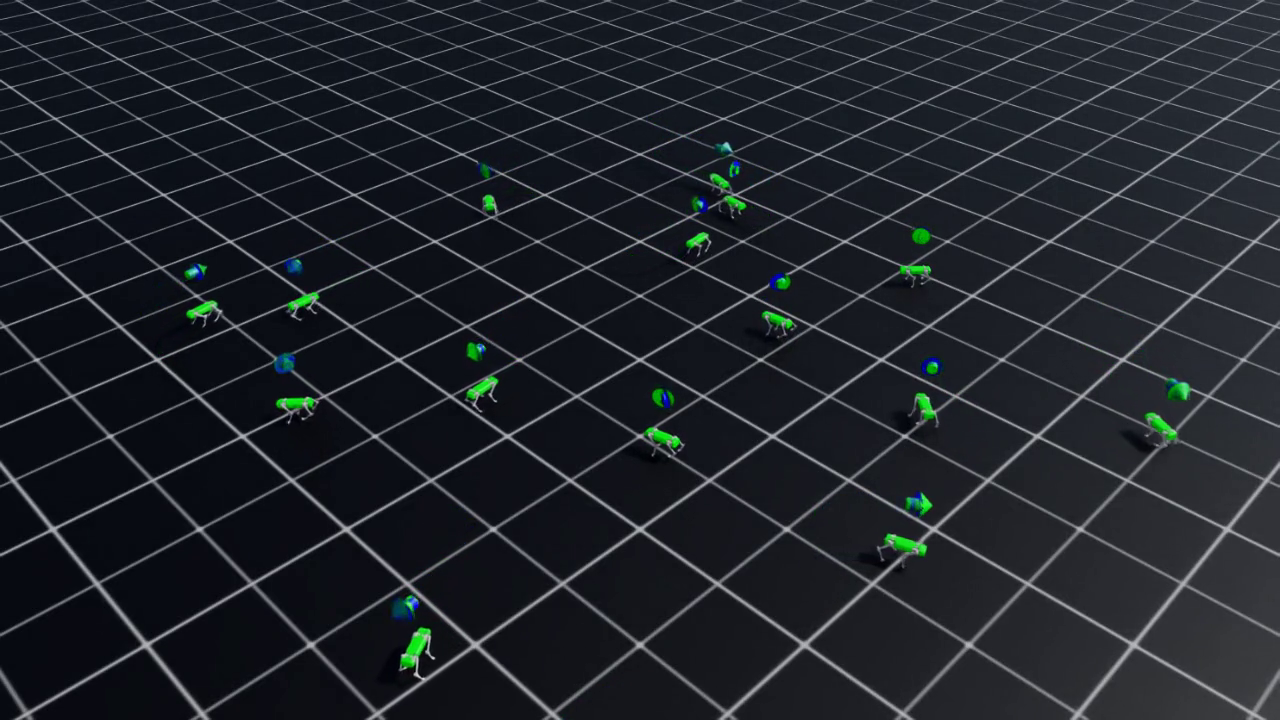
\includegraphics[width=0.72\linewidth]{isaac_walk.png}
\caption{Trained Isaac Lab policy driving multiple Yertle robots in parallel.
Each robot tracks its own commanded velocity.}
\label{fig:isaac_walk}
\end{figure}

\begin{figure}[t]
\centering
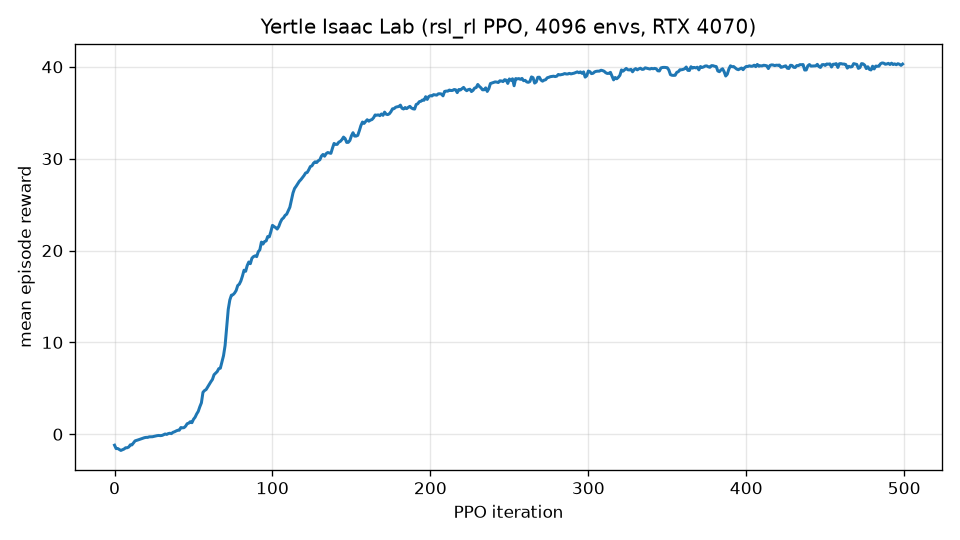
\includegraphics[width=0.78\linewidth]{isaac_reward_curve.png}
\caption{Isaac Lab (rsl\_rl PPO, 4096 environments, RTX 4070) mean episode reward
against training iteration. The policy converges in a few hundred iterations,
about ten minutes of wall-clock time.}
\label{fig:isaac_curve}
\end{figure}

The CPU pipeline, trained from scratch on the same reward, is slower and noisier
but reaches a comparable outcome (Figure~\ref{fig:pybullet_curve}): the resulting
policy walks, tracking commanded forward speeds of around
\SI{0.2}{\meter\per\second}. Its value is as a dependency-light, GPU-free
reference and as the vehicle for the sim-to-real bridge described next.

\begin{figure}[t]
\centering
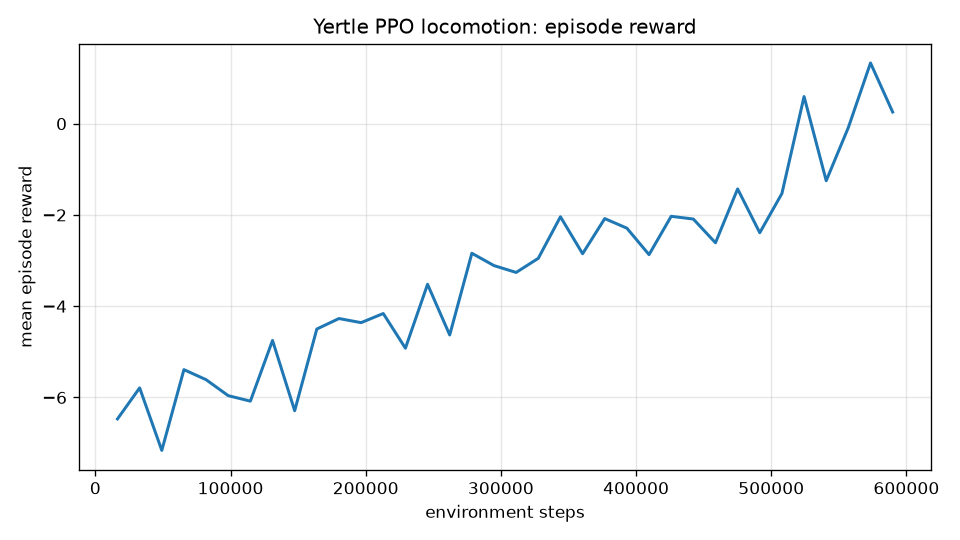
\includegraphics[width=0.78\linewidth]{pybullet_reward_curve.png}
\caption{CPU pipeline (PyBullet, PPO) mean episode reward against environment
steps, showing the same qualitative convergence at far lower throughput.}
\label{fig:pybullet_curve}
\end{figure}

\paragraph{Rough terrain.} The GPU pipeline was also trained on a rough-terrain
task that adds procedurally generated terrain and a height scanner to the
observation. The policy learns to walk over blocks and slopes while keeping the
robot upright for nearly the full episode (Figure~\ref{fig:isaac_rough}),
demonstrating that the same setup extends to non-flat ground with only a change of
task configuration.

\paragraph{Teacher-student distillation.} The flat policy observes the base
linear velocity, which is available in simulation but not measurable on the
robot. To remove this privileged term, the trained policy was used as a frozen
teacher and a student network was trained by behavior imitation from a
deployable observation set (the same observation minus base linear velocity).
After 300 distillation iterations the student reaches a mean episode reward of
40.4 against the teacher's 40.5, with a mean imitation loss of about
$10^{-3}$: walking performance is preserved without the privileged signal, so
the deployed controller needs only the on-board inertial and joint information.

\begin{figure}[t]
\centering
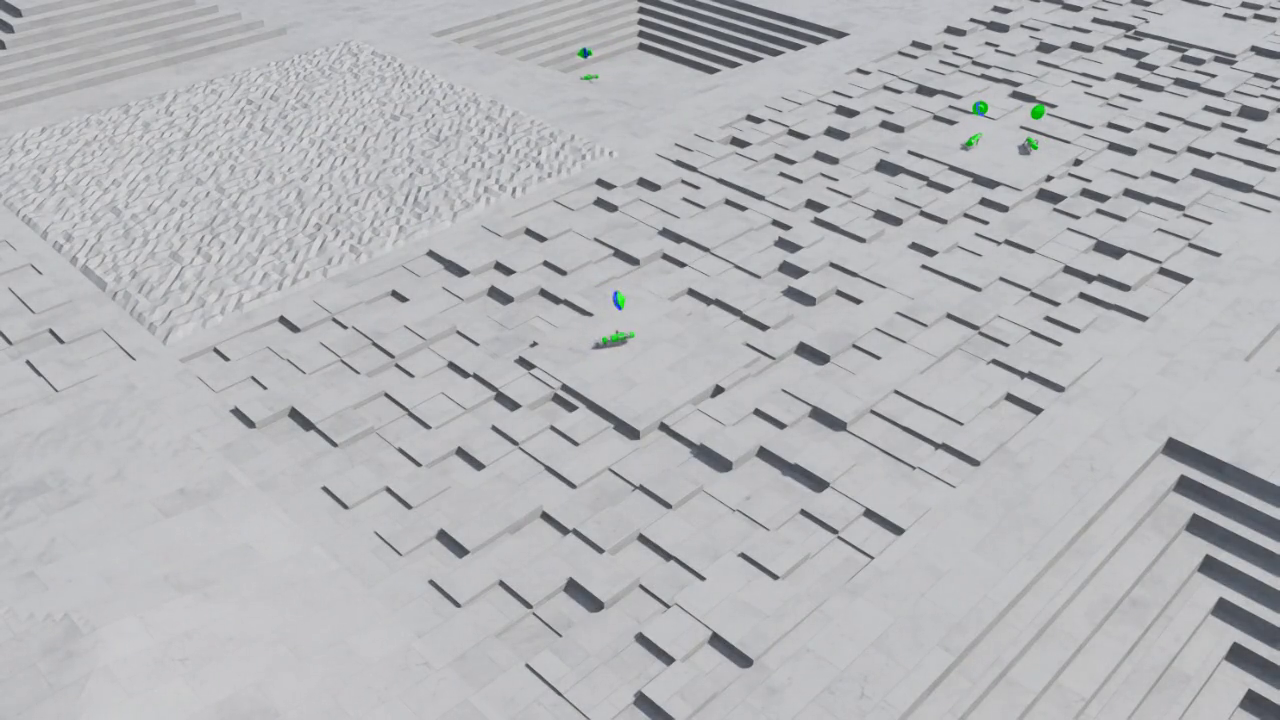
\includegraphics[width=0.82\linewidth]{isaac_rough.png}
\caption{Rough-terrain policy: Yertle robots trained in Isaac Lab walking across
procedurally generated terrain.}
\label{fig:isaac_rough}
\end{figure}

\section{Deployment}
\subsection{Sim-to-real bridge}
A deployment module runs a trained policy at the control rate and converts its
output into firmware joint commands. The observation builder and policy
controller mirror the training environment exactly, and a joint-mapping layer
translates policy targets into the servo convention. Two interfaces are provided:
a PyBullet interface that closes the loop in simulation for validation, and a UDP
interface that streams commands to the ESP32 over the existing protocol. One term
in the observation, the base linear velocity, is available in simulation but not
on the robot; the distilled student policy described above removes it, so the
deployed controller runs from measurable signals only.

\subsection{ROS 2 integration}
A ROS 2 node wraps the same tested deployment core. It subscribes to a velocity
command and an inertial-measurement topic and publishes joint targets, so the
learned controller can be driven from the standard ROS 2 tooling and connected to
a \texttt{ros2\_control} stack or a hardware relay. The node was built with
\texttt{colcon} and run on ROS 2 Humble, and the full control loop was
demonstrated over live topics: a simulation node publishes joint states and
inertial data, the policy node tracks a commanded velocity, and the robot walks.

In addition, the GPU simulation itself was exposed on ROS 2. Through Isaac Sim's
ROS 2 bridge (an OmniGraph action graph), the simulator publishes
\texttt{/joint\_states} and a clock and accepts \texttt{/joint\_command}. This
was verified bidirectionally across two independent ROS 2 installations: an
external ROS 2 environment receives all twelve joint states and, publishing a
joint command, moves the simulated robot, whose tracked position is read back
over the same topics.

\section{Engineering Notes}
Beyond the model repair and reward shaping already described, running the GPU
simulator on a Windows workstation required resolving several dynamic-library
conflicts: the deep-learning runtime and the simulator each load their own math
and OpenMP libraries, and the import order had to be controlled to avoid a hard
crash. Long training runs were launched as detached processes so they survive an
interrupted session.

Two further failure modes are worth recording because each looked like a
learning problem and was not. First, when smoothness penalties (action rate,
joint acceleration, body wobble) were increased to improve gait quality, the
per-step reward went negative; since falling terminates the episode, the optimal
policy became falling immediately to stop accumulating penalty, and mean episode
length collapsed from 1000 steps to about 16. Penalty weights must keep the
per-step reward of useful behavior positive. Second, replacing the implicit
position drive with an explicit DC-motor actuator model, nominally closer to a
real servo, made the robot unable to hold its own stance: at hobby-servo gains
the explicitly applied torque is underdamped, and the torque-speed curve removes
torque exactly when recovery velocity is highest, so the legs oscillate against
their joint limits. A zero-action diagnostic (command the standing pose, watch
base height) isolated both problems in minutes, where staring at training curves
had not. These issues are mundane individually but, collectively, are where most
of the real time is spent, and they are the reason the reproducibility scripts in
the repository are worth as much as the environment code.

\section{Conclusion and Future Work}
Yertle demonstrates that the modern learned-locomotion stack is accessible on a
cheap, printable quadruped and a consumer GPU. A velocity-tracking walking policy
is trained in minutes; the privileged observation is removed by teacher-student
distillation with no loss of performance; and the controller is connected to the
robot's firmware through a deployment bridge, a ROS 2 node running the full loop
over live topics, and a bidirectional Isaac Sim ROS 2 bridge. The simulation
model carries the firmware's joint limits and actuator effort and velocity caps,
which constrain learned behavior to what the hardware can execute. Immediate
future work is to close the sim-to-real loop on the physical robot and to
identify a stable measured actuator model. The code, trained artifacts, and
reproduction scripts are available in the project repository.

\printbibliography

\end{document}
